\documentclass[a4paper,11pt,UTF8]{article}
\usepackage{ctex}
\usepackage{amsmath,amsthm,amssymb,amsfonts}
\usepackage{amsmath}
\usepackage[a4paper]{geometry}
\usepackage{graphicx}
\usepackage{microtype}
\usepackage{siunitx}
\usepackage{booktabs}
\usepackage[colorlinks=false, pdfborder={0 0 0}]{hyperref}
\usepackage{cleveref}
\usepackage{esint} 
\usepackage{graphicx}
\usepackage{ragged2e}
\usepackage{pifont}
\usepackage{extarrows}
\usepackage{mathptmx}
\usepackage{float}
\usepackage{caption}
\captionsetup[figure]{name={Figure}}

\title{Microelectronics Circuit Analysis and Design Homework(7th)}
\author{Yuejin Xie \quad U202210333}
\date{Sept 28th, 2023}
\begin{document}
\maketitle
\noindent4.36 The parameters of the circuit in Figure P4.36 are $R_S = 4 k\Omega$, $R_1 = 850 k\Omega$,
$R_2 = 350 k\Omega$, and $R_L = 4 k\Omega$. The transistor parameters are $V_{T P} = -1.2 $V,
$k^\prime_p = 4 \mu\mathrm{A/V}^2, W/L = 80$, and $\lambda =0.05 \mathrm{V}^{-1}$. (a) Determine $I_{DQ}$ and
$V_{SDQ}$ . (b) Find the small-signal voltage gain $A_v = v_o/v_i$ . (c) Determine the small-signal circuit transconductance gain $A_g=i_o/v_i$. (d) Find the small signal output resistance $R$\\
\begin{figure}[H] 
	\centering 
	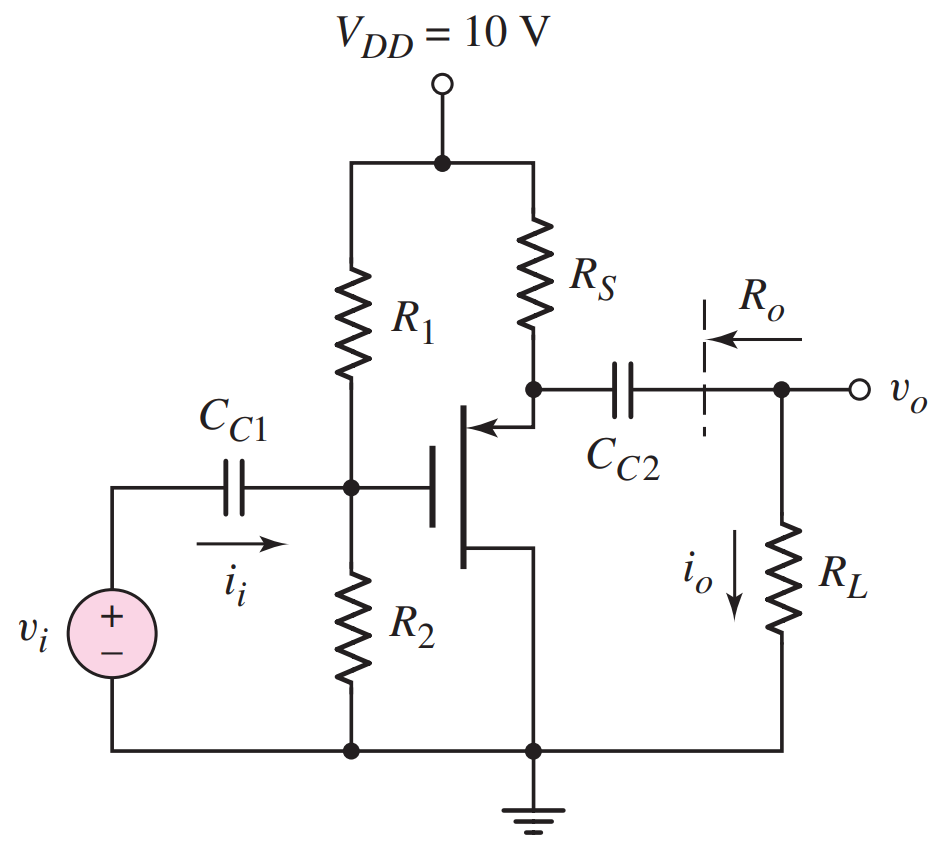
\includegraphics[scale=0.3]{MD4.36.png}
	\caption{Problem 4.36}
\end{figure}
\noindent Solution:\\
It's a PMOS-Enhanced transistor\\
(a)$\displaystyle K_p=\frac{k_p^\prime}{2}\frac{W}{L}=1.6$mA\\
Assume the transistor work in the saturation region, we have equation:
$$
\begin{cases}
	I_{DQ}=K_n(V_{SGQ}+V_{TP})^2\\
	V_S=V_{DD}-I_{DQ}R_S\\
	\displaystyle V_G=\frac{R_2}{R_1+R_2}V_{DD}
\end{cases}\Rightarrow
\begin{cases}
	I_{DQ}=1.25\mathrm{mA}\\
	V_{SDQ}=5\mathrm{V}\\
	V_{SGQ}=2.084\mathrm{V}
\end{cases}
$$
The answer coordinate with the problem.
(b)$g_m=2K_p(V_{SGQ}+V_{TP})=2.828\mathrm{mA/V}, r_o=(\lambda I_{DQ})^{-1}=16\mathrm{k\Omega}$
$R_o=r_o||R_S||R_L=1.778\mathrm{k\Omega}$\\
$\therefore A_v=\frac{g_mR_o}{1+g_mR_o}=0.834$\\
(c)$\displaystyle A_g=\frac{i_o}{v_i}=\frac{i_o}{v_o}\cdot\frac{v_o}{v_i}=\frac{A_v}{R_L}=0.2085\mathrm{mA/V}$\\
\noindent4.40 For the circuit in Figure P4.39, $R_S = 1 k\Omega$ and the quiescent drain current
is $I_{DQ} = 5 \mathrm{mA}$. The transistor parameters are $V_{T N} = -2 $V,
$k^\prime_n = 100\mu \mathrm{A/V}^2$, and $ \lambda = 0.01 \mathrm{V}^{-1}$. (a) Determine the transistor width-to length ratio. (b) Using the results of part (a), find the small-signal voltage gain for $R_L = \infty$. (c) Find the small-signal output resistance $R_o$. (d) Using
the results of part (a), find $A_v$ for $R_L = 2 k\Omega$.\\
\begin{figure}[H] 
	\centering 
	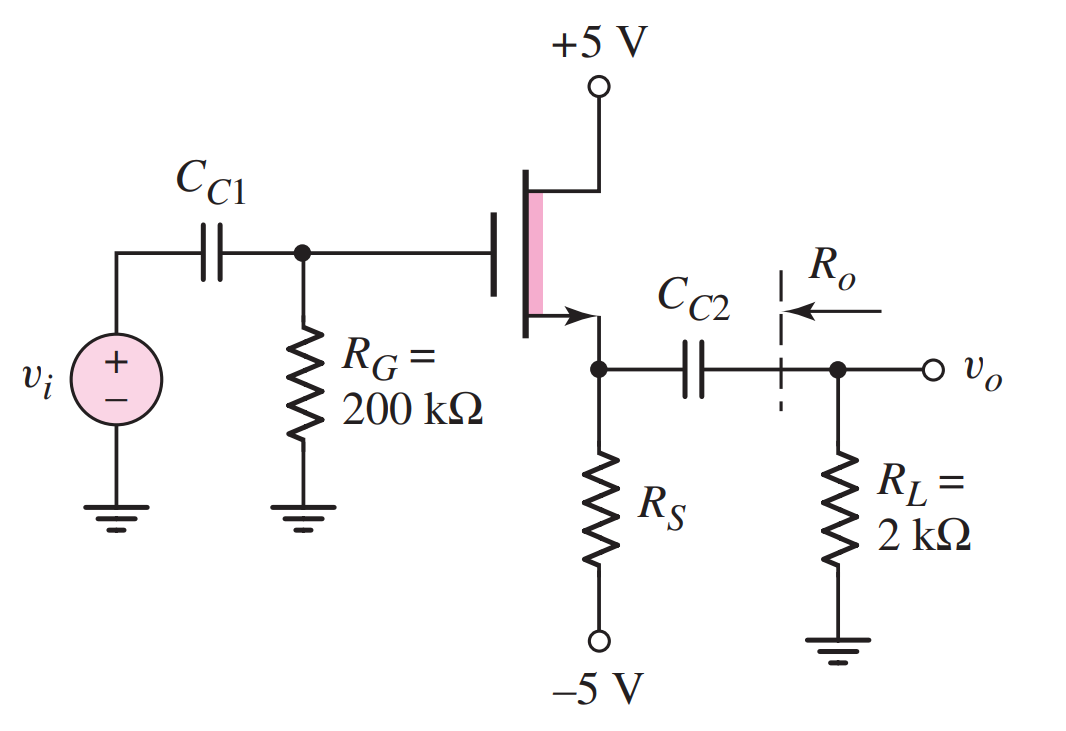
\includegraphics[scale=0.3]{MD4.40.png}
	\caption{Problem 4.40}
\end{figure}
\noindent Solution:\\
Obviously, it's a NMOS-Depletion transistor\\
(a)Assume the transistor works in the saturation region:
$$\begin{cases}
	V_S=V_{SS}+I_DR_S\\
	V_G=0\\
	\displaystyle I_{DQ}=\frac{k^\prime_n}{2}\cdot\frac{W}{L}\\
\end{cases}\Rightarrow\displaystyle \frac{W}{L}=25
$$
(b)$g_m=2\sqrt{K_nI_{DQ}}=5\mathrm{mA/V},r_o=(\lambda I_{DQ})^{-1}=20\mathrm{k\Omega}$\\
$\displaystyle A_v=\frac{g_m(r_o||R_s)}{1+g_m(r_o||R_S)}=0.826$\\
(c)$\displaystyle R_o=\frac1{g_m}||r_o||R_S=165\Omega$\\
(d)$\displaystyle A_v=\frac{g_m(r_o||R_S||R+L)}{1+g_m(r_o||R_S||R+L)}=0.763$\\\\
\noindent4.45 Figure P4.45 is the ac equivalent circuit of a common-gate amplifier. The
The transistor parameters are $V_{TN}=0.4$ V, $k_n^{\prime}=100$ $\mu \mathrm{A/V}^2$ , and $\lambda=0.$The quiescent drain current is $I_{DQ}=0.25$ mA. Determine the transistor $W/L$ ratio and the value of $R_D$  such that the small-signal voltage gain is  $A_v=V_o/V_i=20$ and the input resistance is $R_i=500\Omega$.
\begin{figure}[H] 
	\centering 
	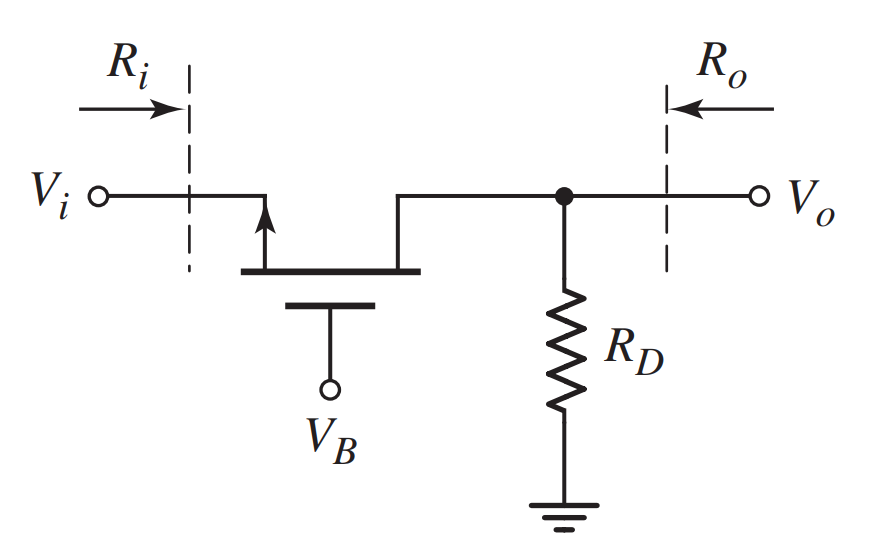
\includegraphics[scale=0.3]{MD4.45.png}
	\caption{Problem 4.45}
\end{figure}
\noindent Solution:\\
$\displaystyle R_i=\frac1{g_m}=0.5\mathrm{k\Omega}\Rightarrow g_m=2\mathrm{mA/V}=2\sqrt{\frac{k_n^\prime}{2}\cdot\frac{W}{L} {I_{DQ}}}\Rightarrow \frac{W}{L}=80$\\
$\displaystyle A_v=\frac{g_mR_D}{1+g_mR_{Si}}=g_mR_D=20\Rightarrow R_D=10\mathrm{k\Omega}$\\
\noindent4.48 For the common-gate circuit in Figure P4.48, the NMOS transistor parameters are:$V_{TN}=1\mathrm{V}$ , $K_n=3 \mathrm{mA/V}^2$, and $\lambda=0$. (a)Determine $I_{DQ}$ and $V_{DSQ}.$
(b)Calculate $g_m$ and $r_o$ (c) Find the small- signal voltage gain $A_v=v_o/v_i.$  \\
\begin{figure}[H] 
	\centering 
	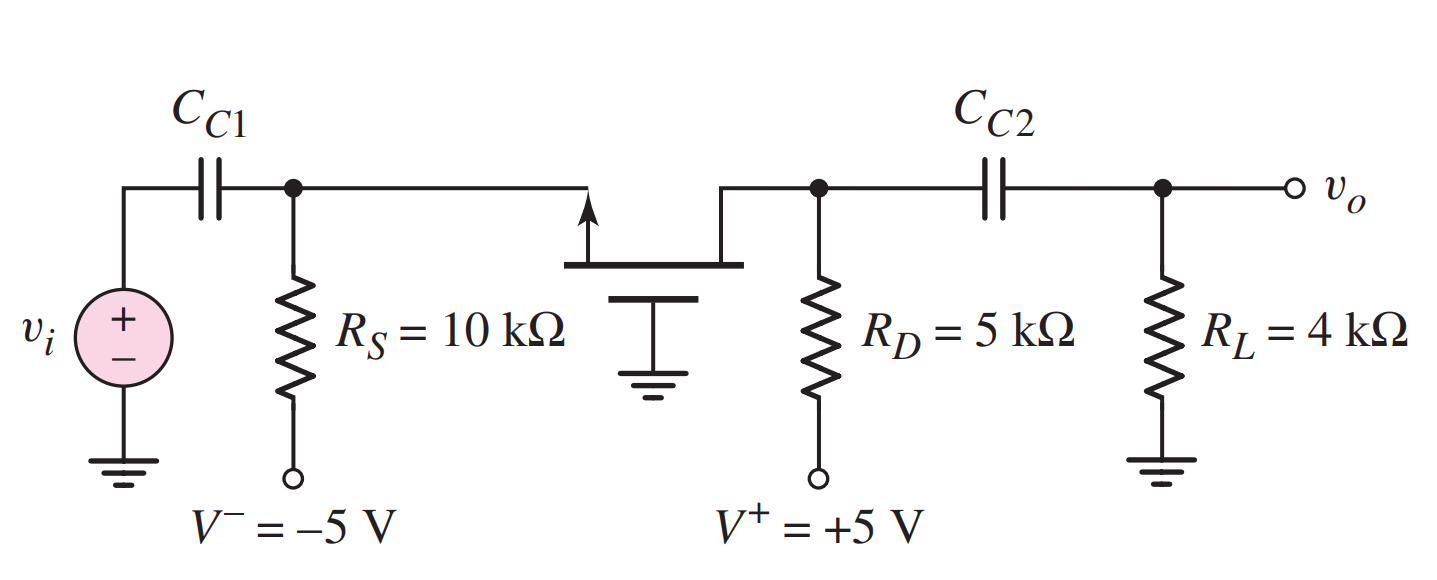
\includegraphics[scale=0.3]{MD4.48.png}
	\caption{Problem 4.48}
\end{figure}
\noindent Solution:\\
Assume the transistor works in the saturation region, we have equations:
$$\begin{cases}
	V_{GS}+I_{DQ}R_S=0-V^-\\
	I_{DQ}=K_n(V_{GS}-V_{TN})^2
\end{cases}\Rightarrow
\begin{cases}
	V_{GS}=1.35\mathrm{V}\\
	I_{DQ}=0.365\mathrm{mA}
\end{cases}
$$
$V_{DSQ}=(V^+-I_{DQ}R_D)-(V^-+I_{DQ}R_S)=4.53\mathrm{V}$\\
(b)$g_m=2K_n(V_{GSQ}-V_{TN})=2.093\mathrm{mA/V},r_o=\infty$\\
(c)$A_v=g_m(R_D||R_L)=4.65$
\end{document}